\documentclass{beamer}
\usepackage[utf8x]{inputenc}
\usepackage[ngerman]{babel}
\usepackage{amsmath}
\usepackage{amsfonts}
\usepackage{amssymb}
\usepackage{graphicx}
\usepackage{subfigure}
\author{Johannes Hackel und Falco Prescher}
\title{WebSocket}

\usetheme{Ilmenau}
\useoutertheme{split}
\usecolortheme{rose}

\begin{document}

\begin{frame}
\titlepage
\end{frame}

\begin{frame}
\frametitle{Gliederung}
\tableofcontents
\end{frame}

\section{Allgemeines zu Websockets}
\begin{frame}
\frametitle{Allgemeines zu Websockets}
\begin{itemize}
\item Unterstützung von Vollduplexkommunikation über ein TCP basierendes Netwerkprotokoll (IETF-Standard \footnote{\tiny{Internet Engineering Task Force (IETF) http://tools.ietf.org/html/rfc6455}})
\item Transmission Control Protokoll (TCP) = verbindungsorientiertes, zuverlässiges und paketvermitteltes Transportprotokoll
\item Ermöglichung einer bidirektionalen Kommunktion zur Realisierung von Datenaustausch in Computernetzwerken
\item Konzipiert für die Implementation in Webbrowsern und Webservern
\item Lieferung einer API für JavaScript (W3C Standard \footnote{\tiny{World Wide Web Consortium (W3C) http://www.w3.org/TR/2011/WD-websockets-20110419/}})
\end{itemize}
\end{frame}

\section{Verwendungen der Websockets}
\begin{frame}
\frametitle{Verwendungen der Websockets}
\begin{itemize}
\item Facebook, Twitter
\item Chats
\item kollaborative Websites (etherpad)
\item Spiele auf HTML5-Basis
\end{itemize}
\end{frame}

\section{Gründe zur Verwendung von Websockets}
\begin{frame}
\frametitle{Gründe zur Verwendung von Websockets}
\begin{itemize}
\item immer mehr Anwendungen durch Webtechnologien
\item fehlende Echtzeit
\item vorher durch Polling/Long Polling
\item führt zu viel Overhead und Netzwerkauslastung
\end{itemize}
\end{frame}

\begin{frame}
\frametitle{Polling/Long Polling}
\begin{figure}
\subfigure{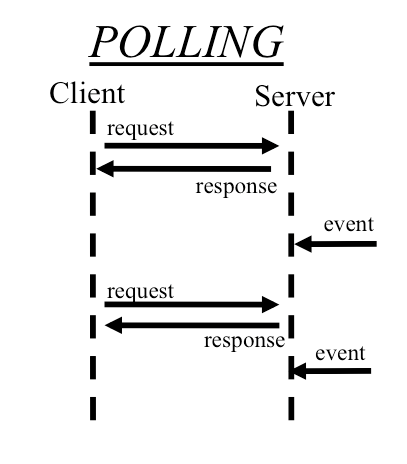
\includegraphics[width=5cm]{polling.png}}
\subfigure{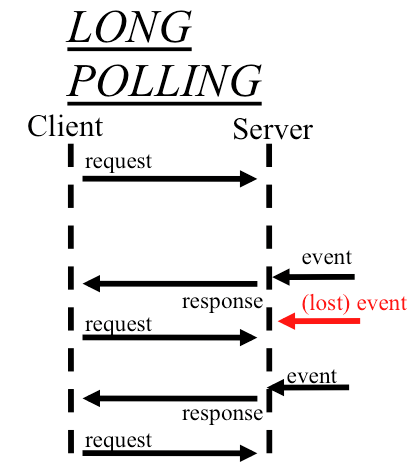
\includegraphics[width=5cm]{long_polling.png}}
\end{figure}
\end{frame}

\begin{frame}
\begin{figure}
\begin{center}
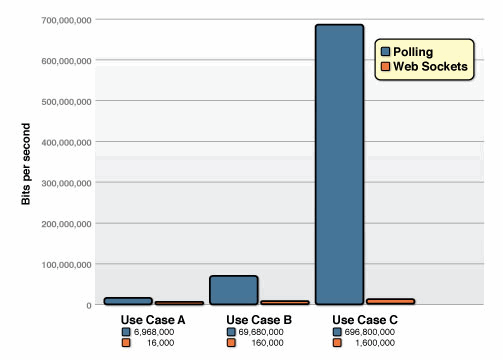
\includegraphics[width=10cm]{poll-ws-compare.png}
\end{center}
\end{figure}
\end{frame}

\section{Bestandteile der Websockets}

\subsection{Netzwerkprotokoll}
\begin{frame}
\begin{figure}[htbp]
\frametitle{Bestandteile}
\framesubtitle{Netzwerkprotokoll}
\begin{minipage}[t]{5cm}
\vspace{0pt}
\begin{itemize}
\item Standard-HTTP-Ports 80 und 443
\item auch durch Firewalls hinweg
\item Verbindungsaufbau durch WebSocket Protocol Handshake
\end{itemize}
\end{minipage}
\hfill
\begin{minipage}[t]{5cm}
\vspace{0pt}
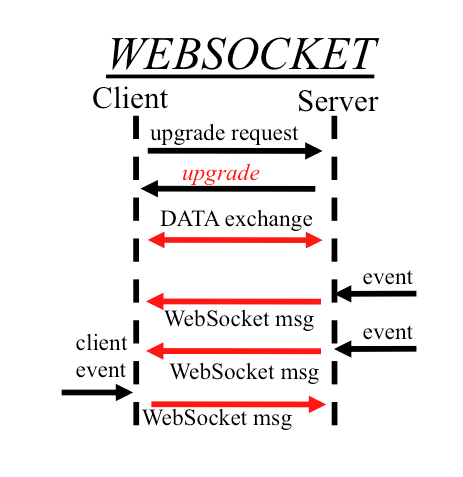
\includegraphics[width=6cm]{WebSocket.png}
\end{minipage}
\end{figure}
\end{frame}

\begin{frame}
\frametitle{Verbindungsaufbau}
\framesubtitle{Client}
GET /chatService HTTP/1.1\\
Host: server.example.com\\
Upgrade: websocket\\
Connection: Upgrade\\
Sec-WebSocket-Key: dGhlIHNhbXBsZSBub25jZQ==\\
Sec-WebSocket-Origin: http://example.com\\
Sec-WebSocket-Protocol: chat, superchat\\
Sec-WebSocket-Version: 8 \\
\end{frame}

\begin{frame}
\frametitle{Verbindungsaufbau}
\framesubtitle{Server}
HTTP/1.1 101 Switching Protocols\\
Upgrade: websocket\\
Connection: Upgrade\\
Sec-WebSocket-Accept: s3pPLMBiTxaQ9kYGzzhZRbK+xOo=\\
Sec-WebSocket-Protocol: superchat\\
\end{frame}

\begin{frame}
\frametitle{WebSocket Protocol}
\begin{itemize}
\item geringer Overhead (zwei Byte)
\item Begin: 0x00
\item Ende: OxFF
\item Daten in UTF-8
\item Beispiel: \textbackslash 0x00Hello, WebSocket\textbackslash 0xff
\end{itemize}
\end{frame}

\subsection{Standardisierte JavaScript Client-API für Websockets}
\begin{frame}
\frametitle{Erstellung der Websocketverbindung vom Client zum Server}
\begin{itemize}
\item // Erstelle neuen Verbindung mit dem Websocket-Server \\
var mySocket = new WebSocket("ws://echo.websockets.org:port");
\end{itemize}
\end{frame}

\begin{frame}
\frametitle{Ereignisbehandlung}
\begin{itemize}
\item // Anfügen von Eventlisteners an dem Websocket \\
	mySocket.onmessage = \\function(event) \{ alert("Der Server sagt: " + event.data); \}; \\
mySocket.onopen = function(event) \{...\}; \\
mySocket.onclose = function(event) \{...\}; \\
mySocket.onerror = function(event) \{...\}; \\
\end{itemize}
\end{frame}

\begin{frame}
\frametitle{Kommunikation mit dem Webserver}
\begin{itemize}
\item // Senden von Daten zum Server \\
mySocket.send("Hallo Server!"); \\
\item // Schließen des Websockets \\
mySocket.close(); \\
\end{itemize}
\end{frame}

\section{Technologien zur Anwendung von Websockets}
\begin{frame}
\frametitle{Implementierungen/Technologien}
\framesubtitle{Server}
\begin{itemize}
\item Apache httpd (via "mod\_pywebsocket")
\item Jetty
\item jWebSocket
\item Kaazing WebSocket Gateway
\item Oracle Glassfish 3.1
\item Netty Project
\item Node.js/Socket.io
\end{itemize}
\end{frame}

\begin{appendix}
\begin{frame}
\frametitle{Quellen}
\begin{itemize}
\item \url{http://www.entwickler.de/zonen/portale/psecom,id,101,online,5134,neu,1.html}
\item \url{http://www.heise.de/developer/artikel/WebSocket-Annaeherung-an-Echtzeit-im-Web-1260189.html}
\item \url{http://www.nodejs.org/}
\item \url{http://www.socket.io/}
\item \url{http://www.stackoverflow.com/questions/10805335/facebook-and-socket-io-node-js}
\item \url{http://www.tools.ietf.org/html/rfc6455}
\item \url{http://www.w3.org/TR/2011/WD-websockets-20110419/}
\item \url{http://www.websocket.org}
\end{itemize}
\end{frame}
\end{appendix}

\end{document}